\chapter{Pengelolaan File CSV}
\section{PEMAHAMAN TEORI}
\begin{enumerate}
\item Apa itu fungsi file csv, jelaskan sejarah dan contoh
\subsection{Fungsi file CSV}
Comma Separated Value atau CSV adalah format data yang memudahkan penggunaanya untuk memudahkan pengguna melakukan penginputan data ke database secara sederhana. CSV bisa digunakan dalam standar file ASCII, yang artinya setiap record dipisahkan dengan tanda(,) atau titik koma(;).Format CSV biasanya digunakan oleh perusahaan besar seperti yayasan, sekolah karena merekalah yang memiliki basis data yang sangat besar dalam penggunaan csv yang memungkinkan pencarian data menjadi lebih mudah dengan menggunakan WordPad.File CSV digunakan untuk menyimpan informasi yang dipisahkan oleh koma, bukan menyimpan informasi dalam kolom.Dan jika teks dan angka disimpan dalam file csv maka mudah untuk memindahkannya dari satu program ke program lain.
\subsection{Sejarah}
	IBM Fortran (level H extended) compiler di bawah OS/360 mendukung fomat CSV pada tahun 1972. FORTRAN 77 mendefinisikan penulisannya dimana input atau output menggunakan tanda koma atau spasi untuk pembatas antar data dan penulisan tersebut sudah disetujui pada tahun 1978.
\hfill\break
	Osborne Executive computer yang mengembangkan SuperCalc spreadsheet pada tahun 1983 membuat konvensi kutipan CSV yang memungkinkan string mengandung koma.
\hfill\break
	Inisiatif standardisasi utama \- mentransformasi \"definisi fuzzy defacto\" menjadi definisi yang lebih tepat dan de jure \-adalah pada tahun 2005, dengan RFC4180, mendefinisikan CSV sebagai Tipe Konten MIME. Kemudian, pada tahun 2013, beberapa kekurangan RFC4180 ditangani oleh rekomendasi W3C.
\hfill\break
	Pada 2014 IETF menerbitkan RFC7111 yang menjelaskan aplikasi fragmen URI pada dokumen CSV. RFC7111 menentukan bagaimana rentang baris, kolom, dan sel dapat dipilih dari dokumen CSV menggunakan indeks posisi.
\hfill\break
	Pada 2015 W3C, dalam upaya meningkatkan CSV dengan semantik formal, mempublikasikan draftrekomendasi pertama untuk stadar metadata CSV, yang dimulai sebagai rekomendasi pada bulan Desembertahun yang sama.
\subsection{contoh}
\lstinputlisting[caption = Contoh penggunaan format CSV., firstline=1, lastline=3]{src/teori1.csv}
\item Aplikasi-aplikasi apa saja yang bisa menciptakan file csv
\begin{enumerate}
\item Editor Tekx (Sublime, Notepad, Atom, visual studio code dan lain-lain) 
\item Spreadshett (Microsoft Excel, google spreadsheet,libreOfficecalc dan lain-lain)
\end{enumerate}
\item Jelaskan bagaimana cara menulis dan membaca file csv di excel atau spreadsheet
\begin{enumerate}
\subsection{Menulis File CSV}
\item pertama-tama buka aplikasi microsoft excel, dengan cara klik start dan cari excel kemudian enter
	\begin{figure}[H]
			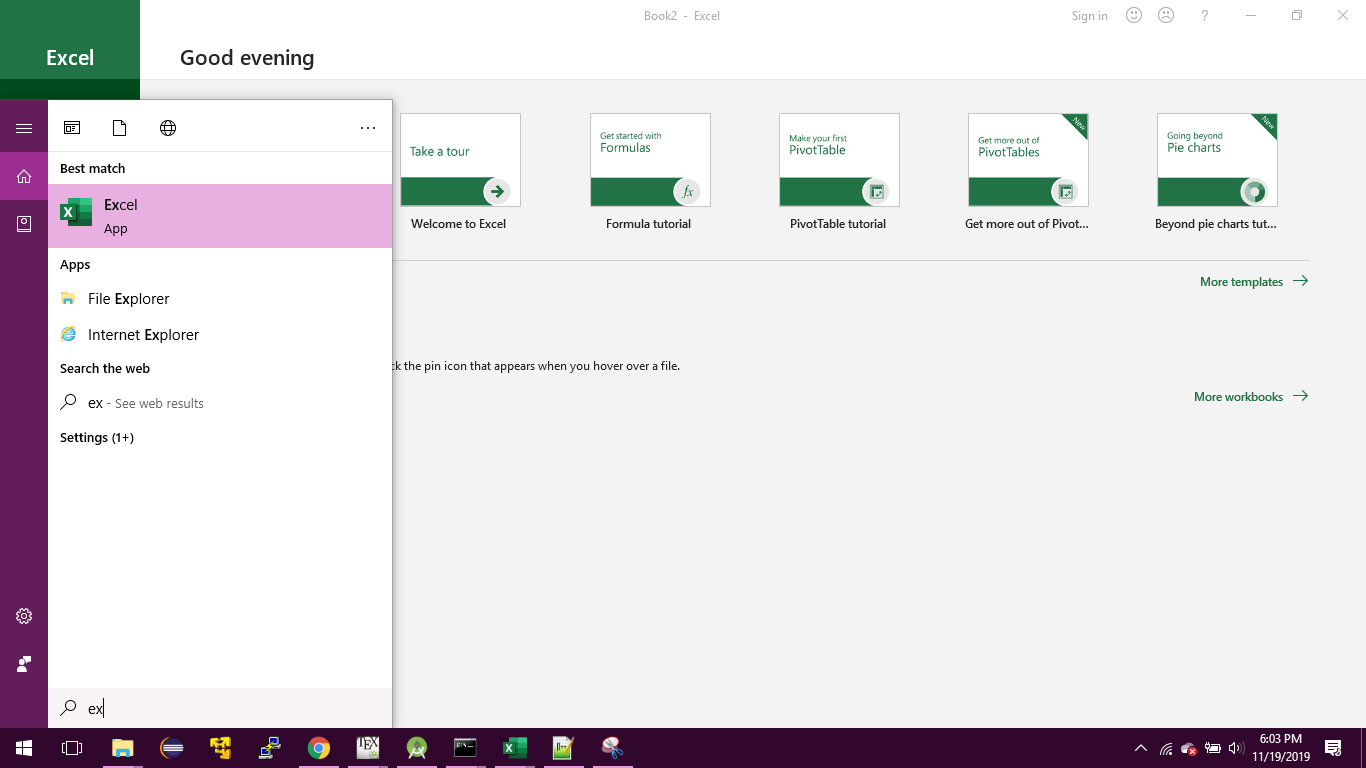
\includegraphics[width=4cm]{figures/1184065/1.png}
			\centering
			\caption{Klik start lalu cari excel}
	\end{figure} 
\item setelah aplikasi microsoft excel terbuka lalu klik Blank Workbokk
 	\begin{figure}[H]
			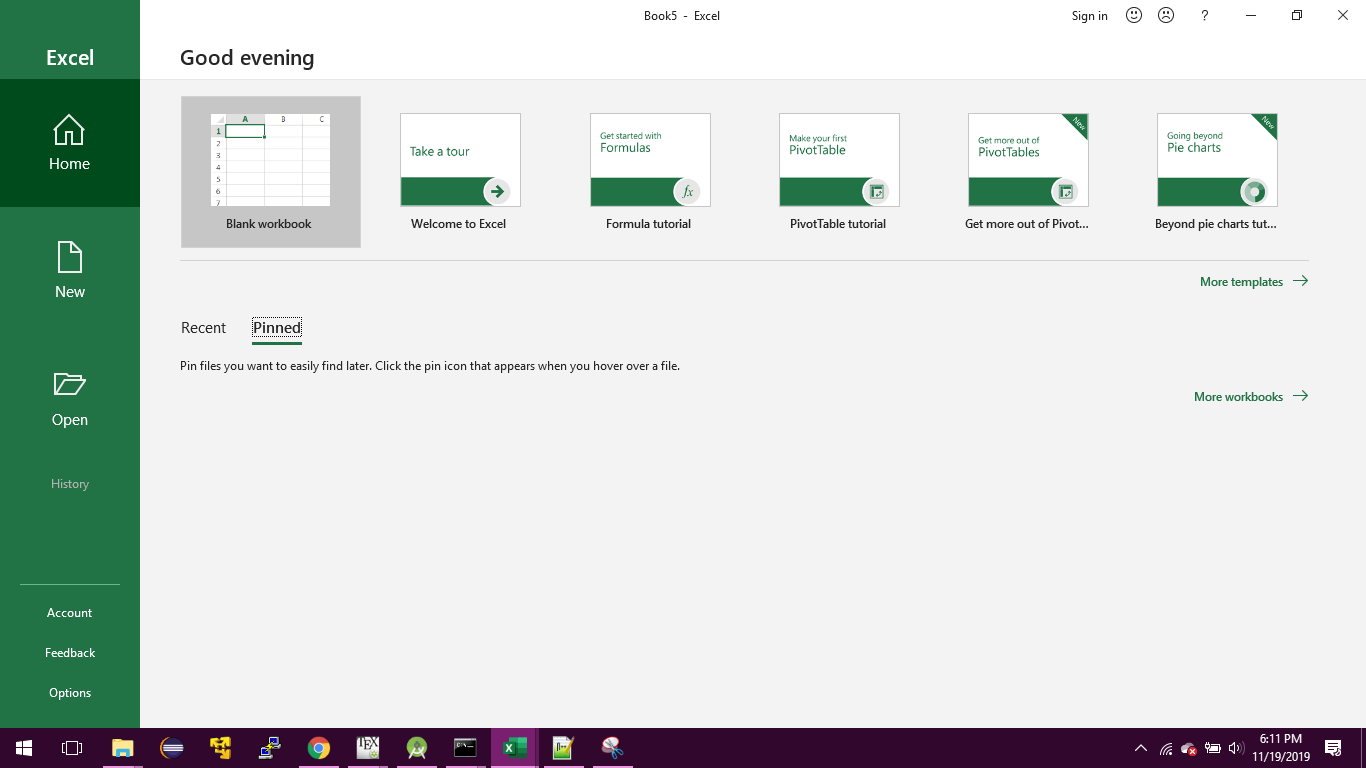
\includegraphics[width=4cm]{figures/1184065/2.png}
			\centering
			\caption{Klik Blank Workbook}
	\end{figure} 
\item setelah Blank Workbook terbuka tulis sesuai data yang diinginkan 
 	\begin{figure}[H]
			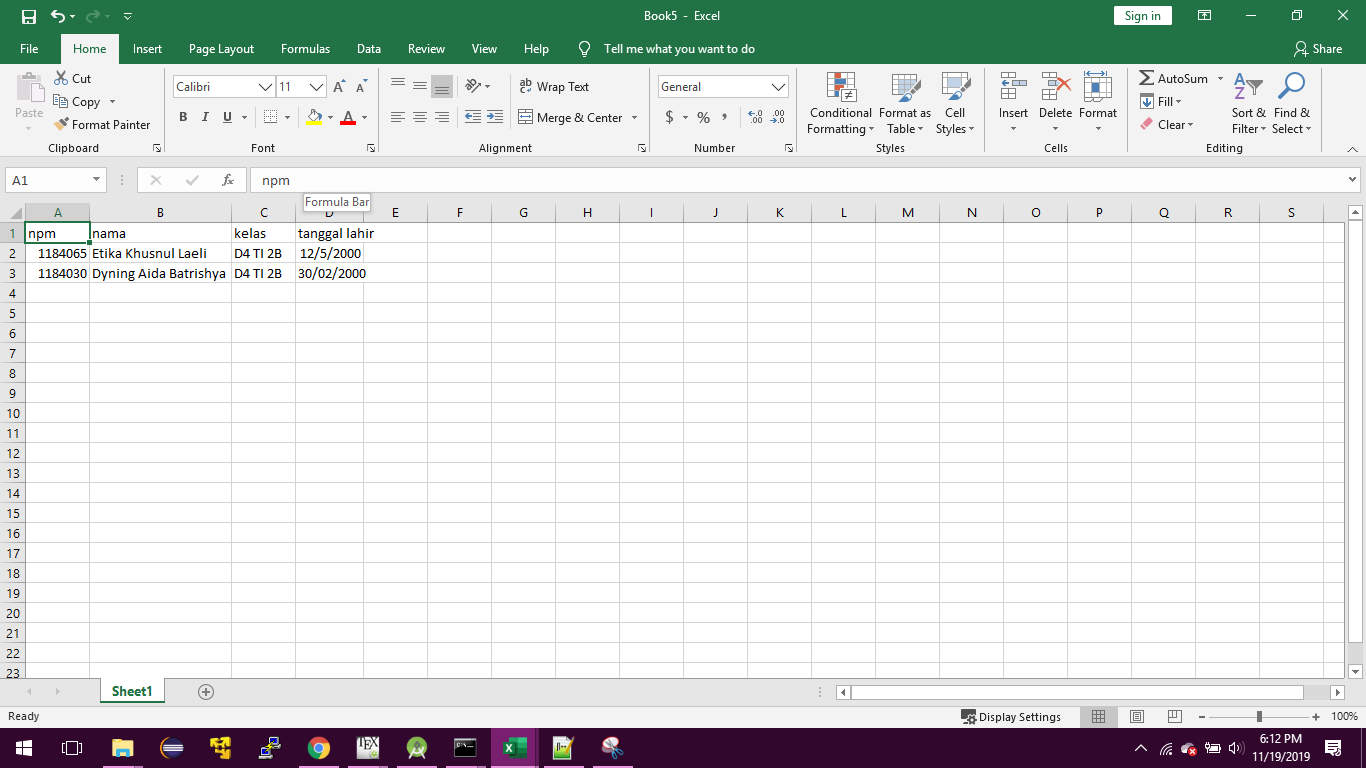
\includegraphics[width=4cm]{figures/1184065/3.png}
			\centering
			\caption{Tulis sesuai data yang diinginkan}
	\end{figure} 
\item setelah data selesai dibuat maka save file tersebut dengan cara klik file lalu save as dan piih browse
 	\begin{figure}[H]
			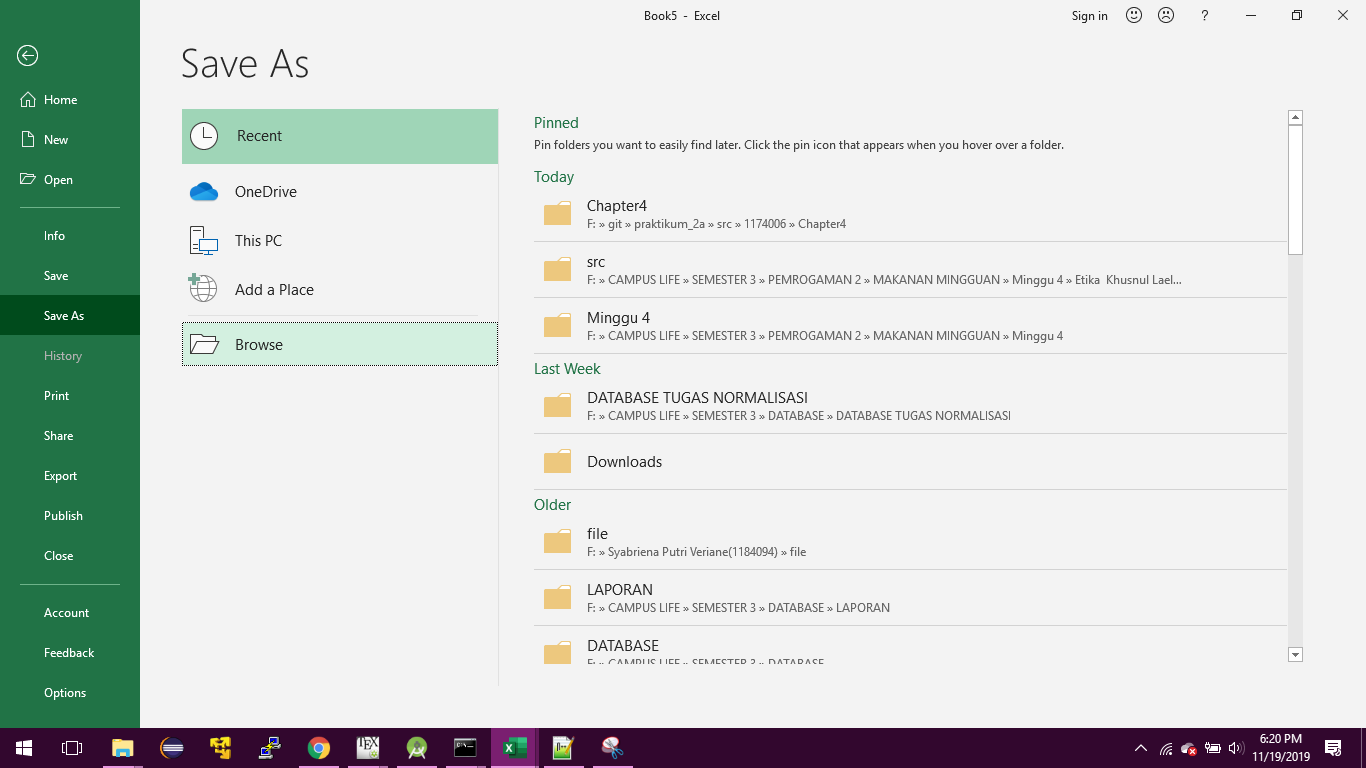
\includegraphics[width=4cm]{figures/1184065/4.png}
			\centering
			\caption{Pilih save as kemudian pilih browse}
	\end{figure} 
\item Kemudian beri nama data filenya pada File Name dan ubah type file pada Save as type menjadi .csv
 	\begin{figure}[H]
			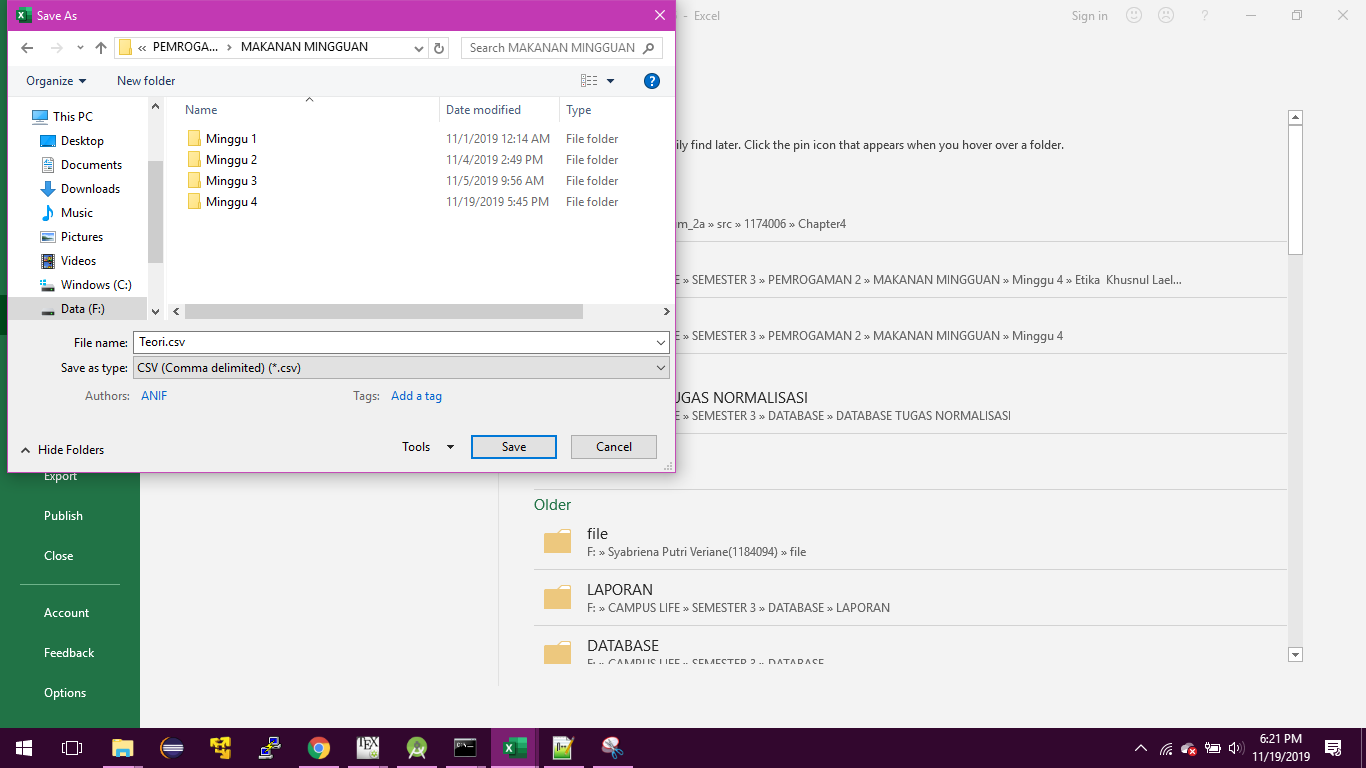
\includegraphics[width=4cm]{figures/1184065/5.png}
			\centering
			\caption{Beri nama file dan ubah save as type nya}
	\end{figure}
\item Kemudian klik save
 	\begin{figure}[H]
			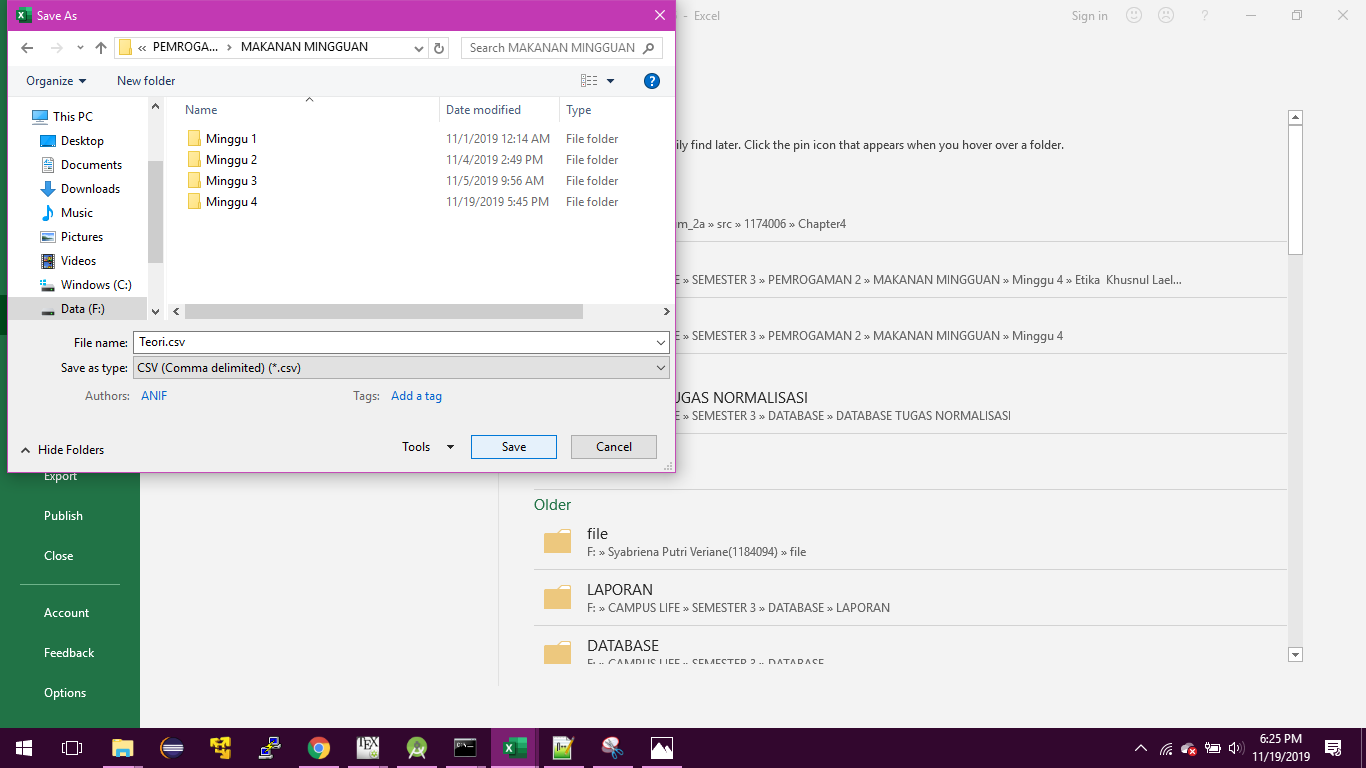
\includegraphics[width=4cm]{figures/1184065/6.png}
			\centering
			\caption{Klik save}
	\end{figure} 
\item Kemudian file yang telah dibuat tadi tersimpan dengan ekstensi .csv. Dan untuk melihat isi filenya tinggal klik dua kali pada file tersebut.
	\begin{figure}[H]
			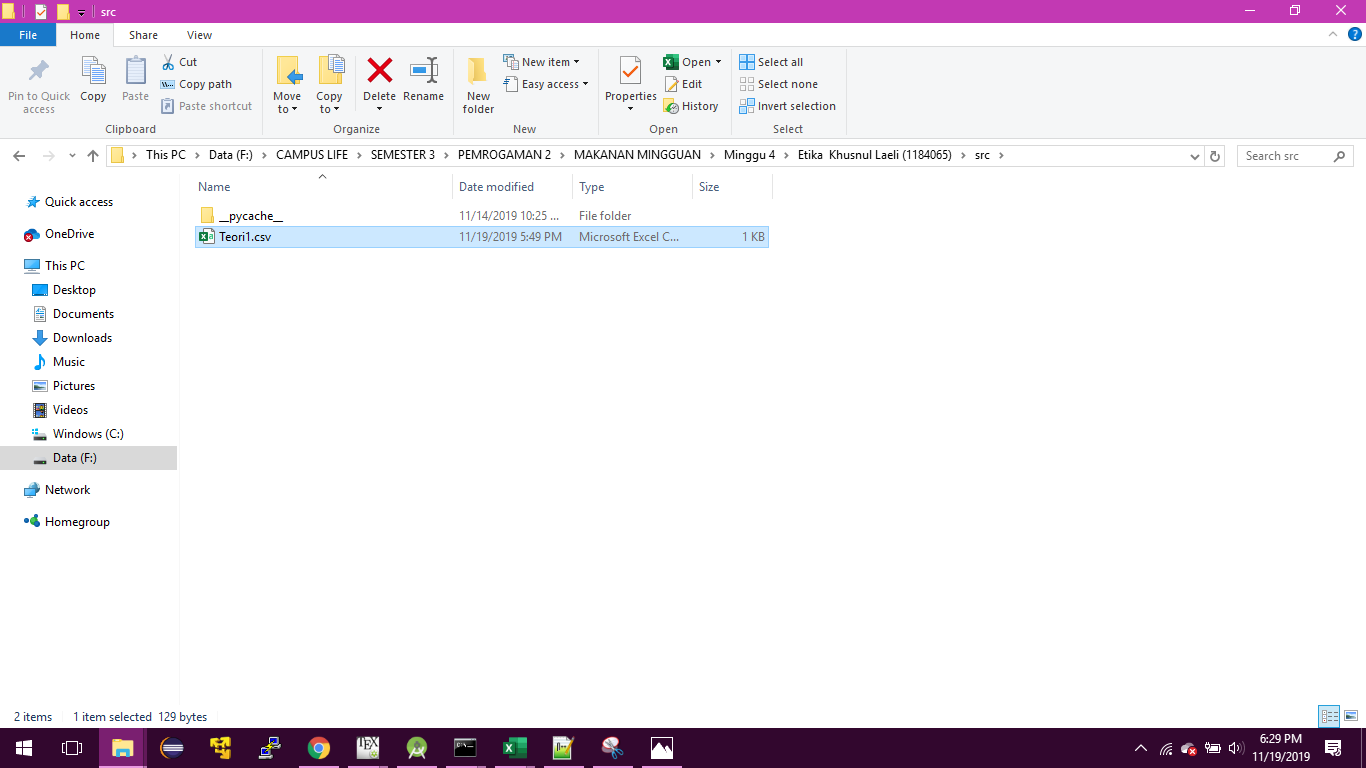
\includegraphics[width=4cm]{figures/1184065/7.png}
			\centering
			\caption{Data berhasil dibuat}
	\end{figure}
\item Ini merupakan isi file yang telah dibuat
	\begin{figure}[H]
			
\includegraphics[width=4cm]{figures/1184065/8.png}
			\centering
			\caption{isi file yang telah dibuat}
	\end{figure}
\subsection{Melihat File CSV di Excel atau Spreadsheet}
\item Pertama klik dua kali pada file yang yang berekstensi CSV.
	\begin{figure}[H]
			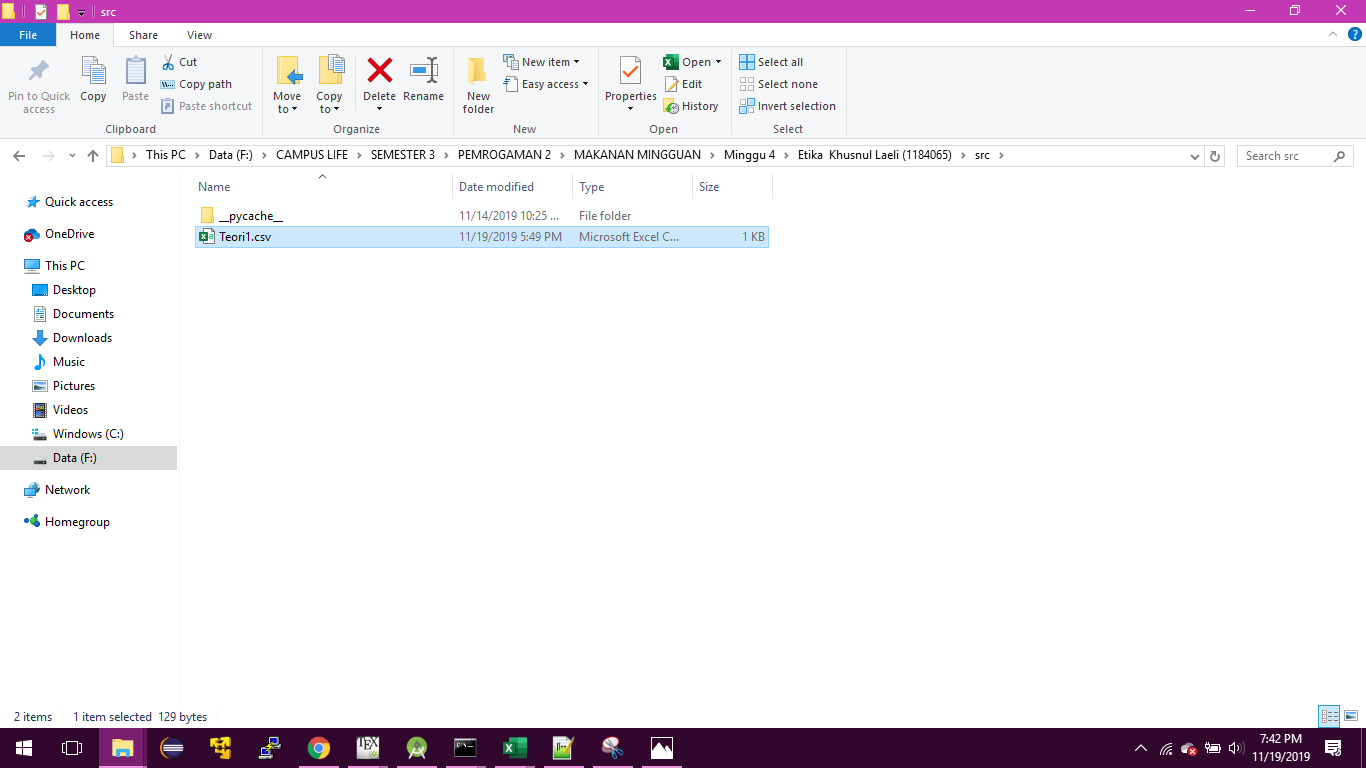
\includegraphics[width=10cm]{figures/1184065/9.png}
			\centering
			\caption{Klik dua kali file berekstensi .csv}
	\end{figure}
\item Kemudian file akan terbuka secara otomatis di aplikasi Excel atau spreadsheet.
	\begin{figure}[H]
			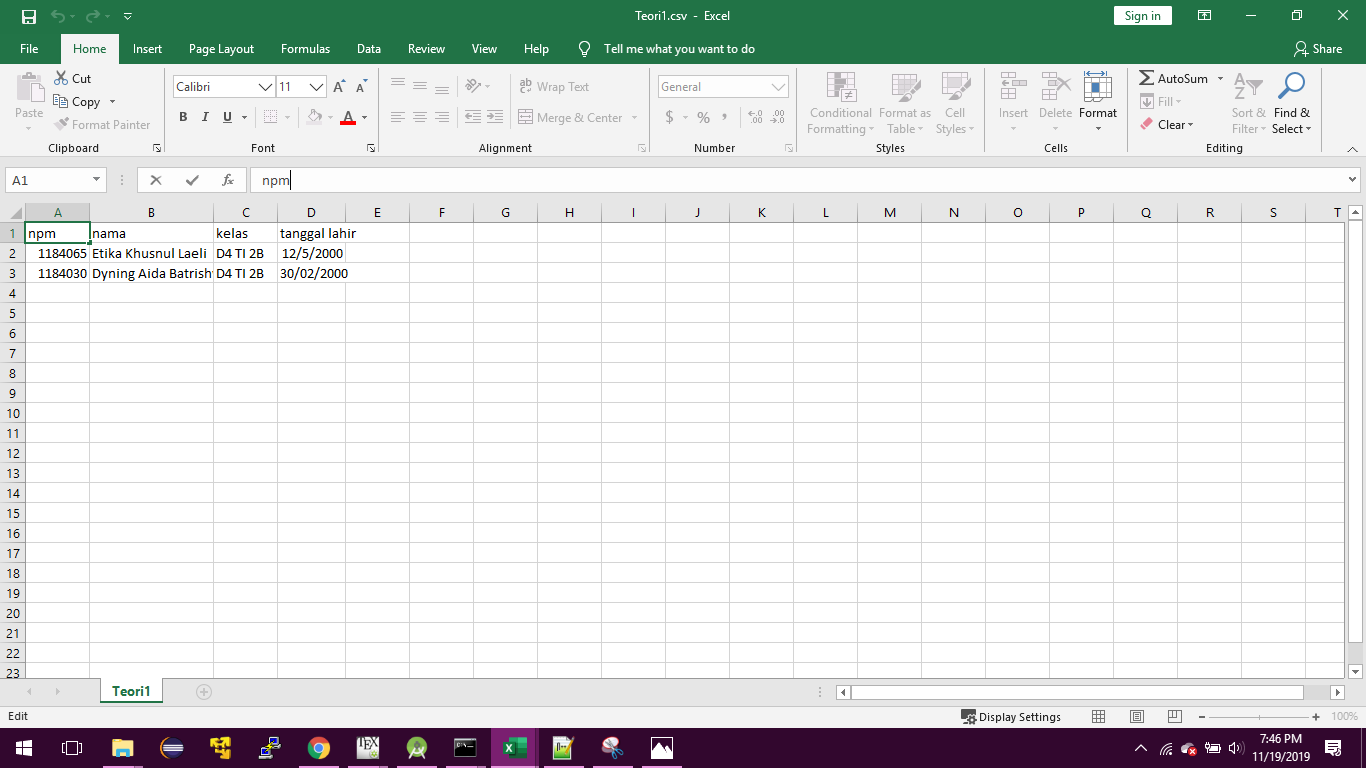
\includegraphics[width=10cm]{figures/1184065/10.png}
			\centering
			\caption{Isi data yang telah dibuat}
	\end{figure}
\end{enumerate} 
\item Sejarah library csv
\hfill\break
Library csv mengimplementasikan kelas yang digunakan untuk membaca dan menulis data dalam format csv. Ini memungkinkan programmer untuk mengatakan "baca data dari file ini yang dihasilkan oleh Excel". Pemrogram juga bisa menentukan format csv sesuai dengan keinginan mereka sendiri.
\item sejarah library pandas
\hfill\break
Pengembangan pandas dumulai pada tahun 2008 di AQR Captal Management. Pandas pada akhir 2009 telah menjadi open source dan secara aktif didukung oleh komunitas individu yang berpikiran sama di seluruh indonesia yang menyumbangkan waktu dan energi mereka untuk membuat pandas bersifat open source mnjadi mungkin. 
\hfill\break
Pandas adalah proyek yang di sponsori oleh NumFOCUS sejak 2005. Ini akan sangat membantu untuk memastikan keberjasilan pengembangan pandas sebagi proyek sumber terbuka kelas dunia.
\item Jelaskan fungsi-fungsi yang terdapat di library csv
\begin{enumerate}
\item reader
\hfill\break
	Reader memiliki fungsi digunakan untuk membaca isi file berformat CSV dari list.
	\lstinputlisting[caption = Membaca file berformat CSV list., firstline=1,lastline=14]{src/Teori1.py}
\item DictReader
\hfill\break
	DictReader memiliki fungsi digunakan untuk membaca isi file berformat CSV dari dictionary.
	\lstinputlisting[caption = Membaca file berformat CSV dict., firstline=1,lastline=14]{src/Teori.py}
\item write
\hfill\break
	Write memiliki fungsi digunakan untuk menulis file berformat CSV dari list.
	\lstinputlisting[caption =  Menulis file berformat CSV list., firstline=1, lastline=17]{src/Teori2.py}
\item DictWrite
\hfill\break
	DictWrite memiliki fungsi digunakan untuk menulis file berformat CSV dari dictionary.
	\lstinputlisting[caption =  Menulis file berformat CSV dictionary., firstline=1, lastline=17]{src/Teori3.py}
\end{enumerate}
\item Jelaskan fungsi-fungsi yang terdapat di library pandas
\begin{enumerate}
\item read\_csv
\hfill\break
	Fungsi ini digunakan untuk membaca isi file berformat CSV
	\lstinputlisting[caption =  Membaca file berformat CSV pandas., firstline=1, lastline=12]{src/Teori4.py}
\item to\_csv
\hfill\break
	Fungsi ini digunakan untuk menulis file berformat CSV
	\lstinputlisting[caption =  Menulis file berformat CSV pandas., firstline=1, lastline=13]{src/Teori6.py}
\end{enumerate}
\section{Bukti bebas Plagiarism}
\begin{figure}[H]
			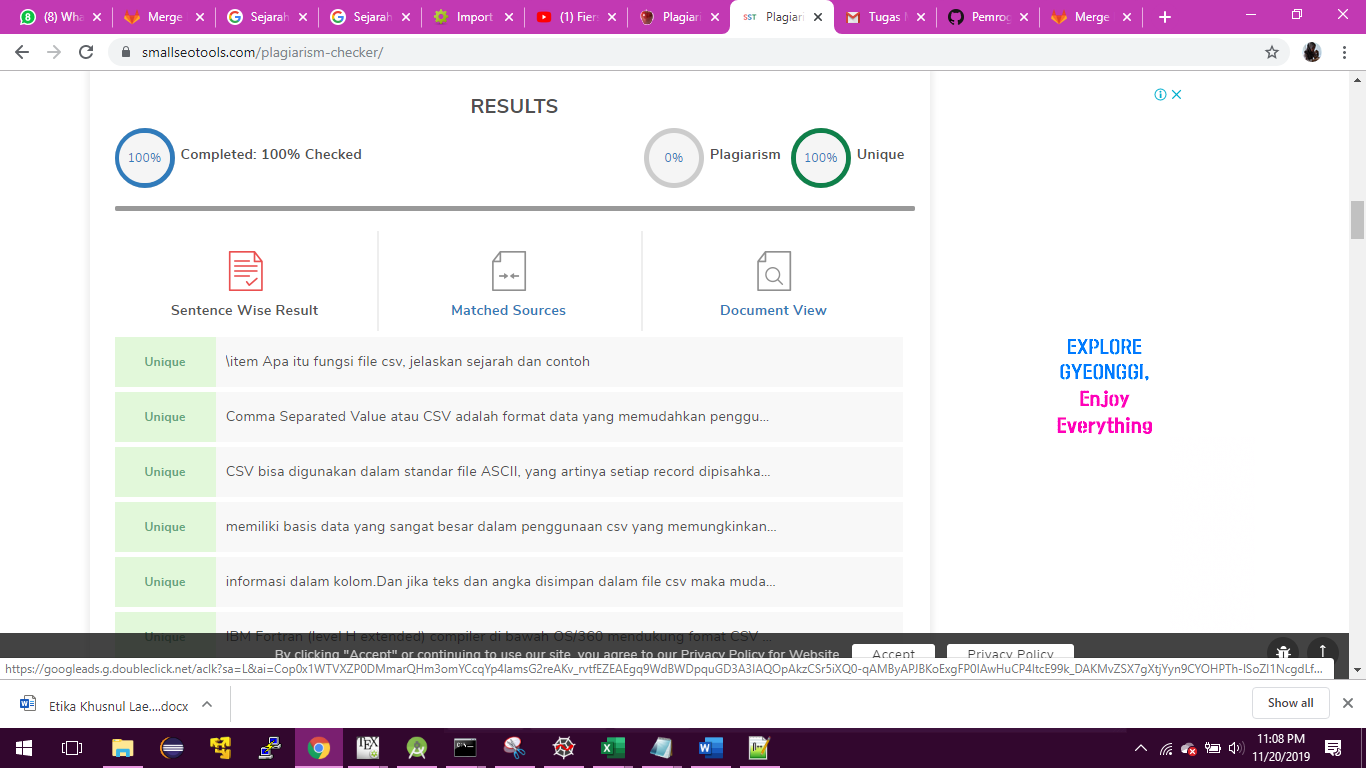
\includegraphics[width=4cm]{figures/1184065/ss1.png}
			\centering
			\caption{Bukti Screenshot bebas plagiarism}
	\end{figure}
\section{Ketrampilan Pemrogaman}
\begin{enumerate}
\item Buatlah fungsi (file terpisah/library dengan NPM\_csv.py) untuk membuka file csv dengan lib csv mode list.
\lstinputlisting[caption =  Membuka Mode List Csv., firstline=1, lastline=13]{src/1184065_csv.py}
\item Buatlah fungsi (file terpisah/library dengan nama NPM\_csv.py) untuk membuka file csv dengan lib csv mode dictionary
\lstinputlisting[caption =  Membuka Mode Dict Csv., firstline=15, lastline=20]{src/1184065_csv.py}
\item Buatlah fungsi (file terpisah/library dengan nama NPM\_pandas.py) untuk membuka file csv dengan lib pandas mode list
\lstinputlisting[caption =  Membuka Mode List Pandas., firstline=1, lastline=13]{src/1184065_pandas.py}
\item Buatlah fungsi (file terpisah/library dengan nama NPM\_pandas.py) untuk membuka file csv dengan lib pandas mode dictionary
\lstinputlisting[caption =  Membuka Mode Dict Pandas., firstline=15, lastline=20]{src/1184065_pandas.py}
\item Buat fungsi baru di NPM\_pandas.py untuk mengubah format tanggal menjadi standar dataframe
\lstinputlisting[caption =  Merubah format Tanggal., firstline=21, lastline=24]{src/1184065_pandas.py}
\item Buat fungsi baru di NPM\_pandas.py untuk mengubah index kolom
\lstinputlisting[caption =  Mengubah Index Kolom., firstline=26, lastline=30]{src/1184065_pandas.py}
\item Buat fungsi baru di NPM\_pandas.py untuk mengubah atribut atau nama kolom
\lstinputlisting[caption =  Merubah Nama Kolom., firstline=32, lastline=36]{src/1184065_pandas.py}
\item Buat program main.py yang menggunakan library NPM\_csv.py yang membuat dan membaca file csv
\lstinputlisting[caption =  Membuat dan membaca file., firstline=1, lastline=13]{src/main.py}
\begin{figure}[H]
			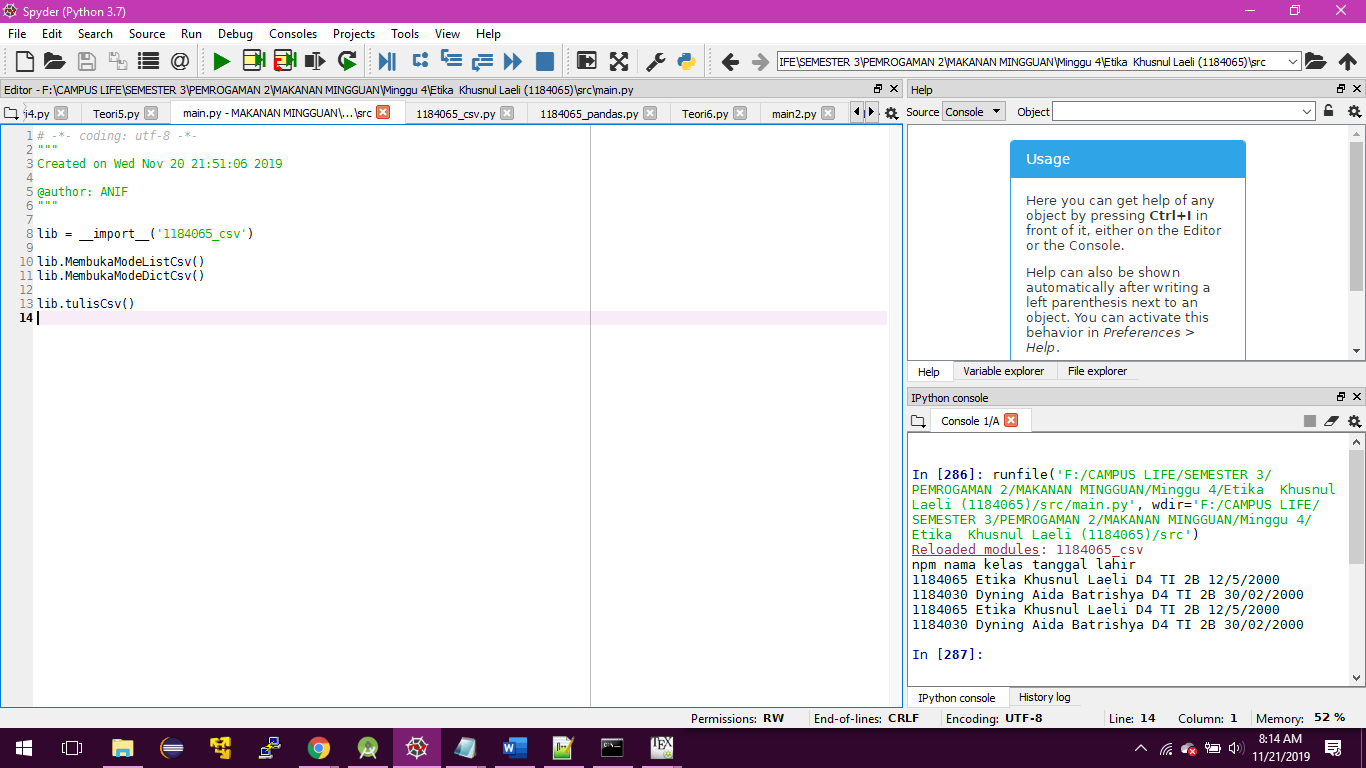
\includegraphics[width=4cm]{figures/1184065/kp1.png}
			\centering
			\caption{Kode Program Main.py}
	\end{figure}
\item Buat program main2.py yang menggunakan library NPM\_pandas.py yang membuat dan membaca file csv
\lstinputlisting[caption =  Membuat dan membaca file., firstline=1, lastline=13]{src/main2.py}
\begin{figure}[H]
			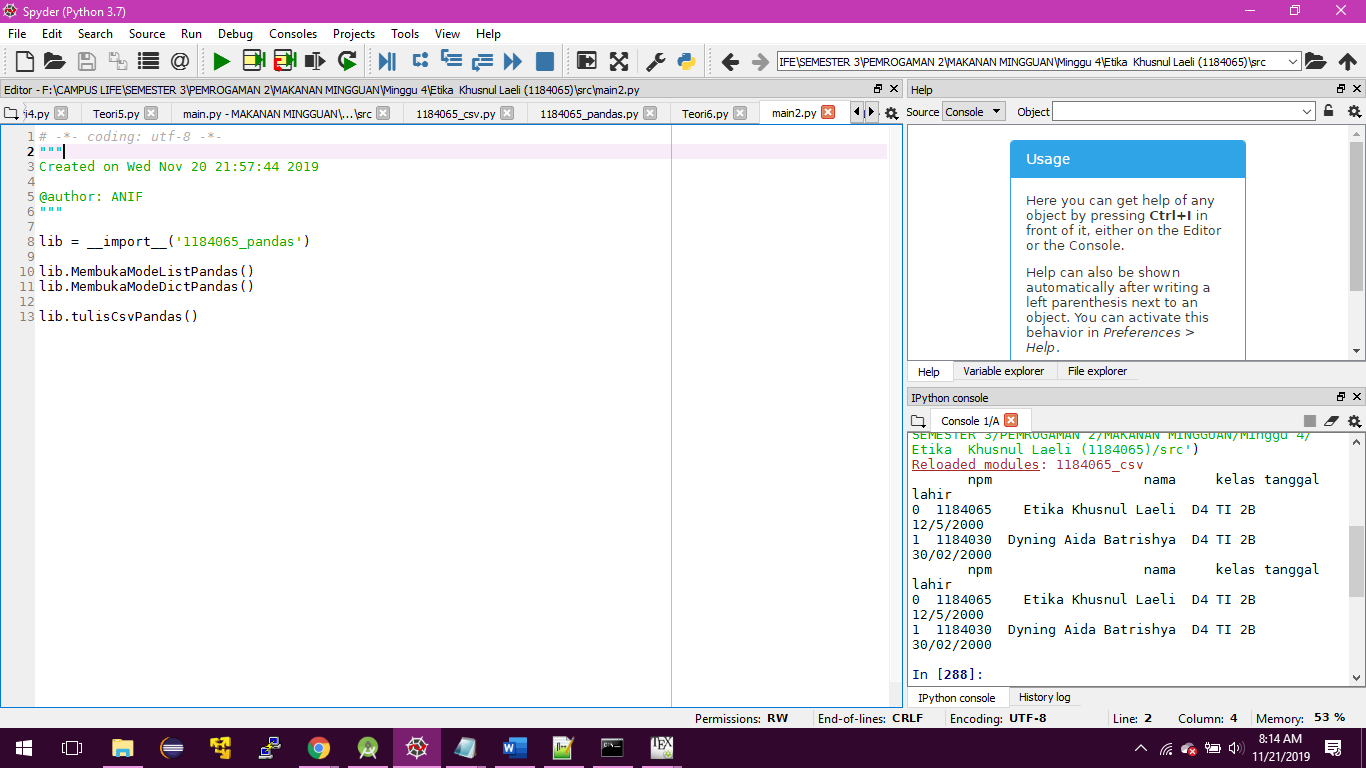
\includegraphics[width=4cm]{figures/1184065/kp2.png}
			\centering
			\caption{Kode Program Main2.py}
	\end{figure}
\end{enumerate}
\section{Bukti bebas Plagiarism}
\begin{figure}[H]
			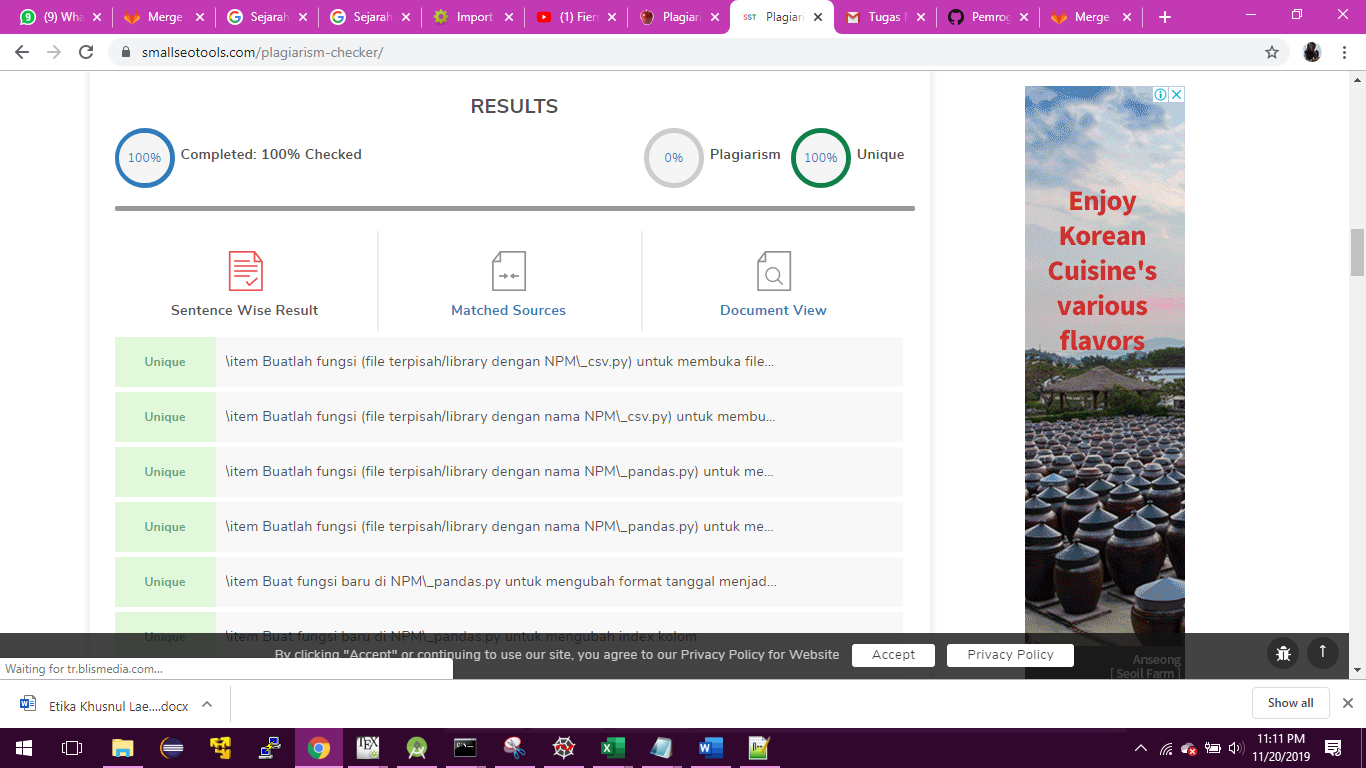
\includegraphics[width=4cm]{figures/1184065/ss2.png}
			\centering
			\caption{Bukti Screenshot bebas plagiarism}
	\end{figure}
\end{enumerate}
\section{Ketrampilan Penanganan Error}
\lstinputlisting[caption =  Fungsi Try Except., firstline=56, lastline=70]{src/1184065.py}
\section{Presentasi Tugas}






